
This part of the development process aims to realize the skeleton of the application and the main functionalities. The output of the process will be and application which offers the possibility to visualize and partially handle todos. It is made of a single page: the HomePage. The HomePage is composed by an AppBar and two tabs: the \textit{todos} tab and the \textit{stats} tab. \\
In the \textit{todos} tab the list of todos is visualized. Is possible to filter todos using a DropdownButton widget in the top right corner, inside the AppBar. 
The available filter values are:
\begin{itemize}
    \item All (visualizes completed and pending todos)
    \item Completed (visualizes completed todo only)
    \item Not Completed (visualizes pending todos only)
\end{itemize}
The list of todos is visualized using a TodoView component widget. The elements that compose the list of todos are called TodoItems. TodoItem widgets visualize the todo’s name and description using two Text widgets and the completion using a Checkbox widget. It is possible to use the checkbox to mark a todo as completed or to mark it as pending depending on its current state. 
In the \textit{stats} tab is possible to visualize the number of completed todos through a Text widget.
In the lower part a TabSelector allow to switch from tabs.

\begin{figure}[H]
    \centering
    \subfloat[\textit{todos} tab runtime UI\label{fig:todos_tab_tree}]{
        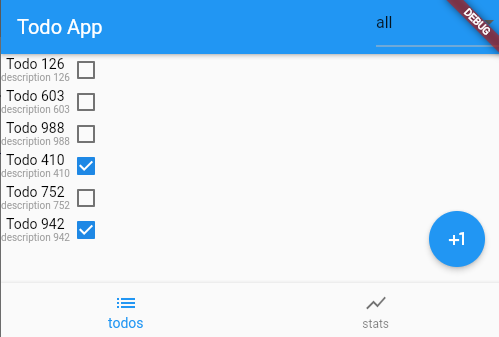
\includegraphics[scale=0.5]{Images/shot_runtime_todoapp_todos.png}
    }
    \quad
      \subfloat[\textit{stats} tab runtime UI.\label{fig:todos_tab_UI}]{
        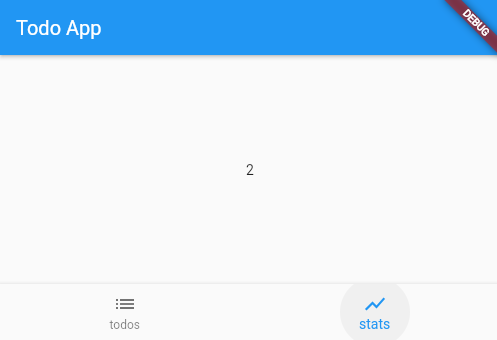
\includegraphics[scale=0.5]{Images/shot_runtime_todoapp_stats.png}
    }
    \caption{Shows the HomePage UI }
    \label{fig:todos_tab}
\end{figure}